\documentclass[12pt,letterpaper]{article}
\usepackage{graphicx,textcomp}
\usepackage{natbib}
\usepackage{setspace}
\usepackage{fullpage}
\usepackage{color}
\usepackage[reqno]{amsmath}
\usepackage{amsthm}
\usepackage{fancyvrb}
\usepackage{amssymb,enumerate}
\usepackage[all]{xy}
\usepackage{endnotes}
\usepackage{lscape}
\newtheorem{com}{Comment}
\usepackage{float}
\usepackage{hyperref}
\newtheorem{lem} {Lemma}
\newtheorem{prop}{Proposition}
\newtheorem{thm}{Theorem}
\newtheorem{defn}{Definition}
\newtheorem{cor}{Corollary}
\newtheorem{obs}{Observation}
\usepackage[compact]{titlesec}
\usepackage{dcolumn}
\usepackage{tikz}
\usetikzlibrary{arrows}
\usepackage{multirow}
\usepackage{xcolor}
\newcolumntype{.}{D{.}{.}{-1}}
\newcolumntype{d}[1]{D{.}{.}{#1}}
\definecolor{light-gray}{gray}{0.65}
\usepackage{url}
\usepackage{listings}
\usepackage{color}

\definecolor{codegreen}{rgb}{0,0.6,0}
\definecolor{codegray}{rgb}{0.5,0.5,0.5}
\definecolor{codepurple}{rgb}{0.58,0,0.82}
\definecolor{backcolour}{rgb}{0.95,0.95,0.92}

\lstdefinestyle{mystyle}{
	backgroundcolor=\color{backcolour},   
	commentstyle=\color{codegreen},
	keywordstyle=\color{magenta},
	numberstyle=\tiny\color{codegray},
	stringstyle=\color{codepurple},
	basicstyle=\footnotesize,
	breakatwhitespace=false,         
	breaklines=true,                 
	captionpos=b,                    
	keepspaces=true,                 
	numbers=left,                    
	numbersep=5pt,                  
	showspaces=false,                
	showstringspaces=false,
	showtabs=false,                  
	tabsize=2
}
\lstset{style=mystyle}
\newcommand{\Sref}[1]{Section~\ref{#1}}
\newtheorem{hyp}{Hypothesis}

\title{Problem Set 1}
\date{Due: February 12, 2023 - Marcus Ó Faoláin, 16327268}
\author{Applied Stats II}


\begin{document}
	\maketitle
	\section*{Instructions}
	\begin{itemize}
	\item Please show your work! You may lose points by simply writing in the answer. If the problem requires you to execute commands in \texttt{R}, please include the code you used to get your answers. Please also include the \texttt{.R} file that contains your code. If you are not sure if work needs to be shown for a particular problem, please ask.
\item Your homework should be submitted electronically on GitHub in \texttt{.pdf} form.
\item This problem set is due before 23:59 on Sunday February 19, 2023. No late assignments will be accepted.
	\end{itemize}

	\vspace{.25cm}
\section*{Question 1} 
\vspace{.25cm}
\noindent The Kolmogorov-Smirnov test uses cumulative distribution statistics test the similarity of the empirical distribution of some observed data and a specified PDF, and serves as a goodness of fit test. The test statistic is created by:

$$D = \max_{i=1:n} \Big\{ \frac{i}{n}  - F_{(i)}, F_{(i)} - \frac{i-1}{n} \Big\}$$

\noindent where $F$ is the theoretical cumulative distribution of the distribution being tested and $F_{(i)}$ is the $i$th ordered value. Intuitively, the statistic takes the largest absolute difference between the two distribution functions across all $x$ values. Large values indicate dissimilarity and the rejection of the hypothesis that the empirical distribution matches the queried theoretical distribution. The p-value is calculated from the Kolmogorov-
Smirnoff CDF:

$$p(D \leq x) \frac{\sqrt {2\pi}}{x} \sum _{k=1}^{\infty }e^{-(2k-1)^{2}\pi ^{2}/(8x^{2})}$$


\noindent which generally requires approximation methods (see \href{https://core.ac.uk/download/pdf/25787785.pdf}{Marsaglia, Tsang, and Wang 2003}). This so-called non-parametric test (this label comes from the fact that the distribution of the test statistic does not depend on the distribution of the data being tested) performs poorly in small samples, but works well in a simulation environment. Write an \texttt{R} function that implements this test where the reference distribution is normal. Using \texttt{R} generate 1,000 Cauchy random variables (\texttt{rcauchy(1000, location = 0, scale = 1)}) and perform the test (remember, use the same seed, something like \texttt{set.seed(123)}, whenever you're generating your own data).\\
	
	
\noindent As a hint, you can create the empirical distribution and theoretical CDF using this code:

\begin{lstlisting}[language=R]
	# create empirical distribution of observed data
	ECDF <- ecdf(data)
	empiricalCDF <- ECDF(data)
	# generate test statistic
	D <- max(abs(empiricalCDF - pnorm(data))) \end{lstlisting}

\vspace{3in}

\section*{Question 1: Answers} 

\noindent Our objective in this question is to generate a function that can successfully calculate the p-value of the Kolmogorov-Smirnov test. We can test the accuracy of our function by testing it against the built-in \texttt{ks.test()} function at the end.
\\\\

\noindent First, we generate 1,000 Cauchy variables:

\begin{lstlisting}[language=R]
data <- rcauchy(1000, location = 0, scale = 1)
\end{lstlisting}

\noindent We can check that they have generated by running:
\begin{lstlisting}
data
\end{lstlisting}

\noindent Next, we can use the hint code to generate the empirical CDF and the test statistic, D:

\begin{lstlisting}
ECDF <- ecdf(data)
empiricalCDF <- ECDF(data)
# generate test statistic
# D = max(|Fo(x) - Ft(x)|)
D <- max(abs(empiricalCDF - pnorm(data)))
D 
\end{lstlisting}

\noindent When run, this gives us an output of \texttt{0.1347281}.
\\\\
\noindent We can now test the data using the built in \texttt{ks.test()} function, which yields the following results:

\begin{lstlisting}
ks.test(data, "pnorm")
\end{lstlisting}

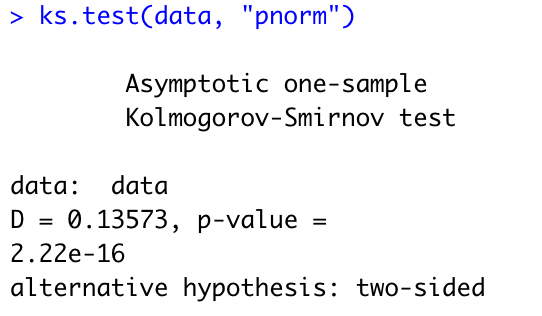
\includegraphics{ks.test.png}

\noindent We can see from this that the p-value is extremely small, at 2.22e-16.
\\\\
\noindent The purpose of the KS test is to see if two data samples come from the same distribution in a two sample test, or in the case of one sample test, to see if a data sample comes from a given fixed distribution, such as the normal distribution.
\\\\
\noindent If the p-value is above our critical $alpha$ value (such as $alpha = 0.05$), then we cannot reject the null hypothesis and conclude that the sample data is from a normal distribution.
\\\\
\noindent If the p-value is below our critical $alpha$ value (such as $alpha = 0.05$), then we reject null hypothesis and must conclude that the data sample was not collected from a normal distribution.
\\\\
\noindent Since our p-value is well below 0.05, we can conclude that the data sample does not come from a normal distribution.
\\\\
\noindent We can now attempt to create our own ks.test function, by attempting to convert the formula from Marsaglia, Tsang and Wang 2003 into R code.
\\\\
\noindent First, we attempt to recreate the mMultiply function from the paper:
\begin{lstlisting}

mMultiply <- function(A, B, C, m){
	i <-0
	j<-0
	while(i<m){
		while(j<m){
			s<-0
			k <-0
			while(k<m){
				s<- s+ A[i*m+k]*B[k*m+j]
				C[i*m+j] <- s
				k<-k+1
			}
			j<-j+1
		}
		i<-i+1
	}
}
\end{lstlisting}

\noindent Next, we attempt to create the mPower function from the paper.

\begin{lstlisting}
mPower <- function(A, eA, V, eV, m, n){
	if(n ==1){
		i<-1
		while(i<m*m){
			V[i] <- A[i]
			eV <-eA
			i<-i+1
		}
		B <- matrix(nrow=m, ncol =m)
		mMultiply(V,V,B,m)
		eB <-2*eV
	}
	if(n%%2==0){
		i <-0
		while(i<m){
			V[i] <- B[i]
			eV <-eB
			i<-i+1
		}
	}
	else{
		mMultiply(A,B,V,m)
		eV <- eA +eB
	}
	if(V[(m/2)*m+(m/2)]>1e140){
		i<-0
		while(i<m){
			V[i]<- V[i]*(1e-140)
			eV <- eV +140
		i<-i+1
		}
	}
return(B)  
}
\end{lstlisting}

\noindent Finally, we attempt to recreate the function K(n, D) function from the paper. 

\begin{lstlisting}
knd <- function(n, d) {
	k <- (n*d) +1
	m <- 2*k-1
	h <- k-n*d
	H <- matrix( nrow=m, ncol = m)
	Q <- matrix( nrow=m, ncol = m)

	i <-0
	j <- 0
	while(i < m) {
		while(j < m) {
			if(i-j+1 <0){
				H[i*m+j]<-0
			}
			else{
				H[i*m+j] <-1
			}
			j <- j+1
		}
		i <- i+1
	}
	i <-0
	while(i <m){
		H[i*m] <- H[i*m] - (h ^ (i+1))
		H[(m-1)*m+1] <- H[(m-1)*m+1] - (h^(m-i))
		i <- i +1
	}
	H[(m-1)*m] <- H[(m-1)*m] + ifelse(2 * h - 1>0, (2*h-1)^m, 0)
	i<-0
	j<-0
	while(i<m){
		while(j<m){
			if(i-j+1 >0){
				g<-1
				while(g<= i-j+1){
					H[i*m+j] <- H[i*m+j]/g
					g<- g+1
				}
			}
			j <- j+1
		}
		i <- i+1
	}
	eH <-0
	mPower(H, eH, Q, m, n)

	s <- Q[(k-1)*m+k-1]
	i<-1
	while(i<=1){
		s<- s*i/n
			if(s<1e-140){
			s<- s*1e140
			eQ <- eQ-140
		}
		i<-i+1
	}
	s<-s*(10^eQ)
	return(s)
}
\end{lstlisting}

\noindent We then test our created function, which generates the following output:
\begin{lstlisting}
knd(1000,D)
\end{lstlisting}

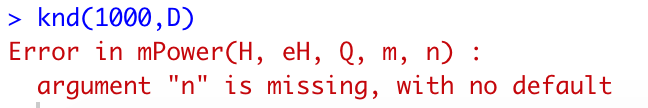
\includegraphics{Error in mPower.png}

\noindent As we can see, the function performs poorly at generating the p-value, giving an error message instead of a p-value.


\pagebreak
\section*{Question 2}
\noindent Estimate an OLS regression in \texttt{R} that uses the Newton-Raphson algorithm (specifically \texttt{BFGS}, which is a quasi-Newton method), and show that you get the equivalent results to using \texttt{lm}. Use the code below to create your data.
\vspace{.5cm}
\begin{lstlisting}[language=R]
set.seed (123)
data2 <- data.frame(x = runif(200, 1, 10))
data2$y <- 0 + 2.75*data2$x + rnorm(200, 0, 1.5)
\end{lstlisting}

\pagebreak

\section*{Question 2 Answers}

\noindent We start off by generating the data as above.

\begin{lstlisting}
set.seed (123)
data2 <- data.frame(x = runif(200, 1, 10))
data2$y <- 0 + 2.75*data2$x + rnorm(200, 0, 1.5)
\end{lstlisting}

\noindent We can inspect the top six observations of the data using the head() function.

\begin{lstlisting}
head(data2)
\end{lstlisting}

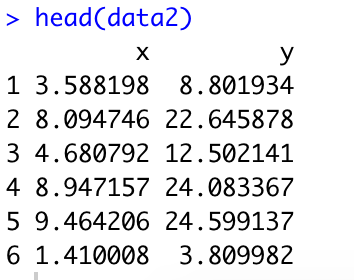
\includegraphics{head(data2).png}

\noindent We start off by estimating the slope and intercept of the data using the linear regression method.

\begin{lstlisting}
q2_lm <- lm(y~x, data = data2)
summary(q2_lm)
\end{lstlisting}

\noindent This function call generates the following output.

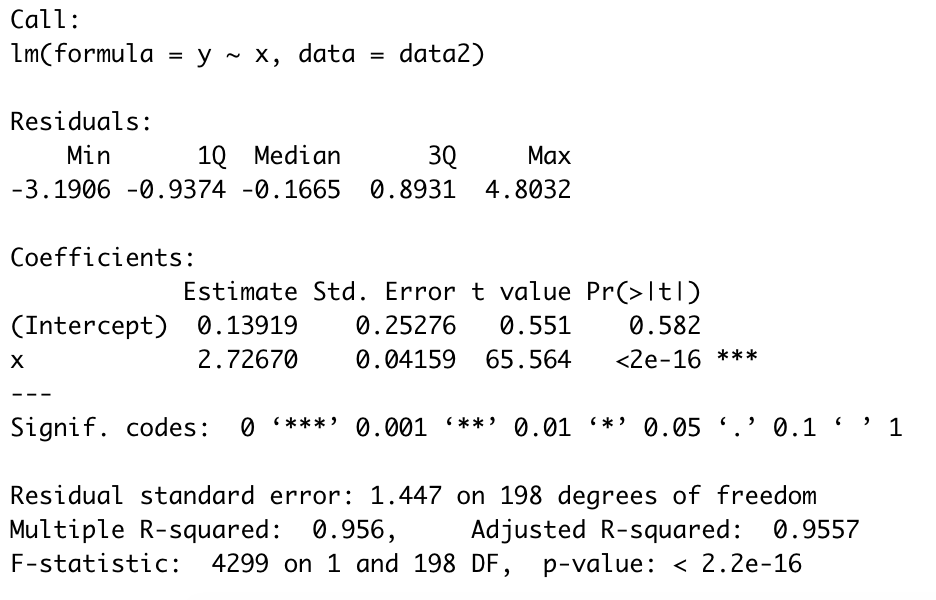
\includegraphics{summary(q2_lm).png}

\noindent As we can see, the linear model gives us an intercept estimate of 0.13919 and a slope estimate of 2.72670.
\\\\

\noindent We must estimate an OLS regression that uses the Newton-Raphson algorithm.
\\\\
\noindent We set up the linear likelihood function that returns the log likelihood of the Maximum likelihood estimate, since the the slope and intercepts values that maximise the log likelihood will also maximise likelihood and is less computationally intensive.

\begin{lstlisting}
linear.lik <- function(theta, y, X){
	n <- nrow(X)
	k <- ncol(X)
	beta <- theta[1:k]
	sigma2 <- theta[k+1]^2
	e <- y - X%*%beta
	logl <- -(0.5)*n*log(2*pi) - (0.5)*n*log(sigma2) - ( (t(e) %*% e)/(2*sigma2))
	return(-logl)
}
\end{lstlisting}

\noindent Next, we can find the values that maximise the log likelihood and therefore return the maximum likelihood intercept and slope values using the \texttt{optim()} function.
\\\\
\begin{lstlisting}
linear.MLE <- optim(fn = linear.lik,
					  par = c(1,1,1),
					  hessian = TRUE,
					  y = data2$y,
					  X = cbind(1, data2$x),
					  method = "BFGS"
)
\end{lstlisting}

\noindent We can get find out the elements of the MLE estimation using \texttt{\$par}.

\begin{lstlisting}
linear.MLE$par
\end{lstlisting}

\noindent When we run this we generate the following output:

\includegraphics{linear.MLE\$par}

\noindent As we can see from the output, we get similar results to the linear model: around 0.1398 for the intercept and around 2.7266 for the slope, which is approximately equivalent to our linear model estimates of 0.13919 for our intercept and 2.72670 for our slope.
\\\\
\noindent This shows that we can generate equivalent results using a linear model as we can with an OLS regression that uses the Newton-Raphson algorithm.

\end{document}
